\documentclass[draftclsnofoot, onecolumn,journal,letterpaper,10pt, compsoc]{IEEEtran}

\usepackage{url}
\usepackage{color}
\usepackage{geometry}
\usepackage{tabularx}
\usepackage{listings}
\usepackage{fancyvrb}
\usepackage{varwidth}
\usepackage{setspace}
\usepackage{float}
\usepackage{graphicx}
\usepackage{pgfgantt}
\graphicspath{ {./images/} }

\geometry{margin=0.75in}   
\singlespacing

\def \TitlePageHeader{Droplet Productions}
\def \TitlePageTitle{Requirements}
\def \GroupNumber{by Group 13}
\def \GroupMembers{James Barry, Tarren Engberg, Dennis Li, James Luo,  Brice Ng}
\def \CourseTitle{CS 461 - Senior Design}
\def \CourseTerm{Fall 2018}

\title{Group13Requirements}
			
\newcommand{\NameSigPair}[1]{\par
\makebox[2.75in][r]{#1} \hfil 	\makebox[3.25in]{\makebox[2.25in]{\hrulefill} \hfill		\makebox[.75in]{\hrulefill}}
\par\vspace{-12pt} \textit{\tiny\noindent
\makebox[2.75in]{} \hfil		\makebox[3.25in]{\makebox[2.25in][r]{Signature} \hfill	\makebox[.75in][r]{Date}}}}
\renewcommand{\NameSigPair}[1]{#1}

%i pull \centerfloat from memoir here, so i can use it for figures
\makeatletter
\newcommand*{\centerfloat}{%
  \parindent \z@
  \leftskip \z@ \@plus 1fil \@minus \textwidth
  \rightskip\leftskip
  \parfillskip \z@skip}
\makeatother

%%%%%%%%%%%%%%%%%%%%%%%%%%%%%%%%%%%%%%%

\begin{document}
\begin{titlepage}
    \pagenumbering{gobble}
    \begin{singlespace}
        \hfill    
        \par\vspace{.2in}
        \centering
        \scshape{
            \huge \TitlePageHeader \par
            {\large\today}\par
            \vspace{.5in}
            \textbf{\Huge \TitlePageTitle }\par
            \vfill
            \vspace{5pt}

            \vspace{5pt}
            {\Large
                \NameSigPair{\GroupNumber}\par
            	\NameSigPair{\GroupMembers}\par
                \NameSigPair{\CourseTitle}\par
                \NameSigPair{\CourseTerm}\par
            }
            \vspace{20pt}
        }
    \end{singlespace}
    \begin{abstract}
    This document covers development requirements for the location-tagging mobile application called Droplet. The requirements have been left intentionally vague by the client, so potential ideas are itemized here. Development will start with documentation, such as the problem statement and tech review. Once the tech options have been evaluated, development will begin on the back-end elements such as the database and internal API, followed by the front-end elements such as the user interface. Once the application is complete, we will begin testing to ensure that it works as intended. A Gantt chart at the end gives a rough view of our planned timelime for the project.
    \end{abstract}
\end{titlepage}

\newpage
\pagenumbering{arabic}
\clearpage

\pagebreak

\section{Project Summary}

In our previous problem statement document, we proposed a location-tagging mobile application called Droplet. Its goal is to bring physical connection to social media by making people explore the world to see posts made by others. Rather than posting to their account, as is typical on social media, users post on a location instead, and only users nearby can view and interact with those posts. When making a post, one can set a "splash radius" (hence the name Droplet), which is the distance in which other users can see their post. People can favorite and comment on posts made by others, assuming they are within this radius. A user can also review all the posts they have made, regardless of where they are, allowing them to chronicle their adventures and memories in a location-based way. 

\section{Logistics}

\subsection{Documentation}
Our first step in development is documentation. So far we have written a problem statement that summarized why this project is being made in the first place. Next is our technology review, which gives us an opportunity to explore options and will inform many of our more technical design decisions later on. After that, we will move into visual design and similar topics, following the class schedule. This will be a constant effort over the course of this project.

\subsection{Technology Review}
The technology review is an extremely important part of our documentation, due to our client leaving our tech requirements intentionally vague. We will research all of the different options available to us when designing our project during this phase. This includes looking at different database structures and technologies, available geographical map APIs, client/server web API standards, front-end frameworks and construction methodologies and many other software approach choices in order to determine what will best serve our project the most.  We plan to thoroughly flesh out any and all specifics about the project during this time to determine which software related frameworks, languages and technologies suit the project's end goals the best.

\subsection{Development Cycle}
We have chosen to use Agile methodologies during the development of our project, given how much freedom we have, so we can iterate and try new things on the fly. Ideally, we will implement a functioning back-end and a prototype for our front end, then iterate on that prototype until we have a product which satisfies the project's minimum viable product specification.

\section{Back End}

\subsection{Database \& Internal API}
After evaluating viable options for our database technology, we will use our database to store user account and post information, including text, video, photos and post meta-data. Our team will have to structure our data into an enhanced entity-relationship (EER) diagram. This diagram allows us to understand how all of the data we have stored is connected. Following the diagram, we will have to create and host the database on a server. After creating the database, we will test storing and fetching data from it.

We will also need to develop an internal API in order to communicate with our database, and will be designed to pull and store requests. This will allow for multi-platform compatibility. 

\subsection{Third-Party APIs}
Having a functioning GPS map is essential to our project, so selecting a good map API is high priority. After researching map APIs, we will choose one the best suits our needs. The map API must be able to accurately display an icon at the user's post location with minimal cost per API call, as well as display the user's location when they look at the map. In addition, the map needs to be accurate enough to differentiate a street or sidewalk from a building with precision.  Having the extra precision in the map API will improve the longevity of the app and possibly allow for future features such as augmented reality.

\section{Front End}

\subsection{User Interface Design}
Concurrent with the back-end construction, we will also be building the user interface. We currently have a few simple mock-ups for design direction to give us an idea of what the client is looking for in terms of design and appearance (pictured below), and we will create more based on the mockups in order to generate a full, exhaustive UI design, while focusing on making sure that the interface is user friendly. This will involve some additional research into usability design. Once we have created a full design that we think will be acceptable in terms of both appearance and usability, we will start testing to see whether or not the designs we come up with are usable by employing user testing with people who have never used the app before. If the design turns out to be unintuitive and too difficult to use, we will iterate on the design before testing again.
\begin{figure}[!htb]
    \centering
    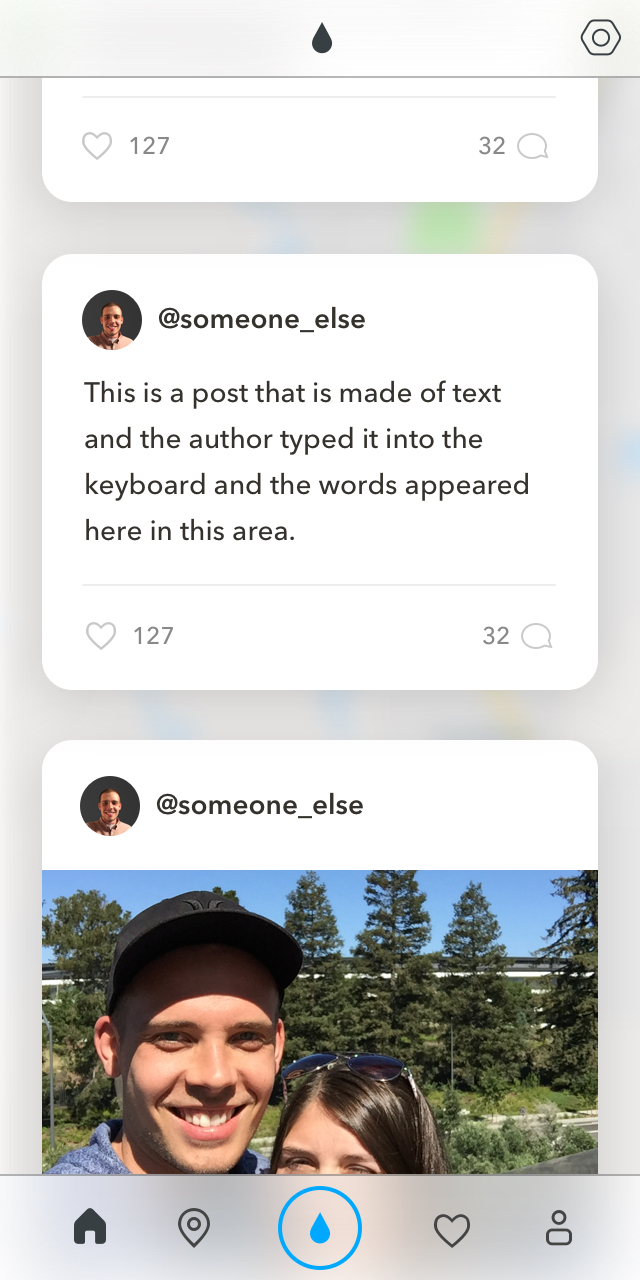
\includegraphics[scale=.25]{home.jpg}
    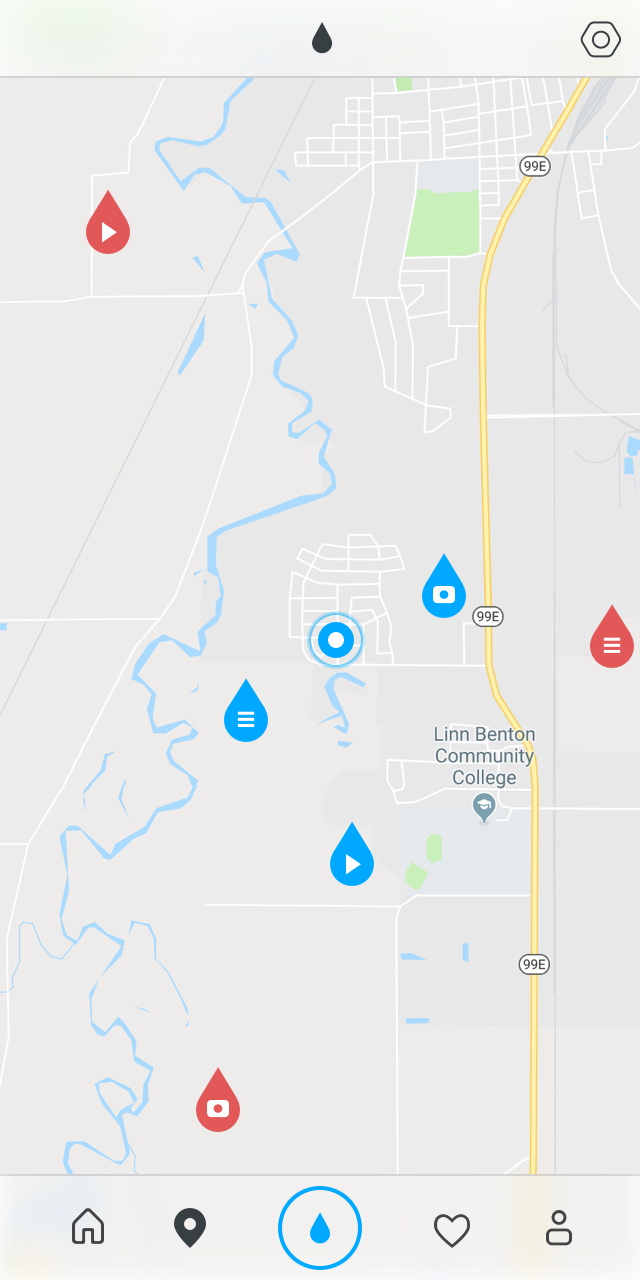
\includegraphics[scale=.25]{maps.jpg}
    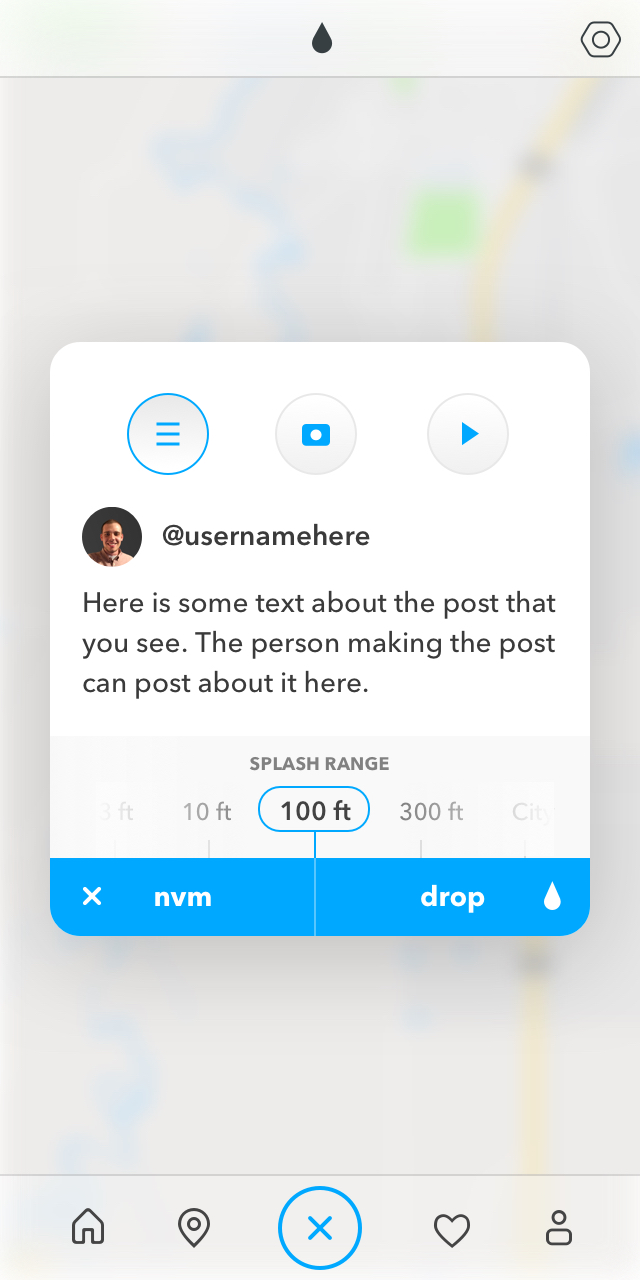
\includegraphics[scale=.25]{new_droplet.jpg}
    \caption{Initial user interface design mockups}
    \label{fig:my_label}
\end{figure}

\section{Functionality Testing}
Once the majority of the application has been completed, we will shift over to testing. We will be testing individual parts of the app as we go, but this will serve as a way to confirm that the app works as a whole. We will perform extensive testing to ensure that it works to the standard expected by the client. Thus, we will not only test for functionality, but also for aspects such as speed, usability, etc. 

We will test early and often. Using testing frameworks, we will design our unit tests at the same time that we are designing our functions and classes so that the building blocks of the application (both front-end and back-end) are solid before we even begin integration testing. Once the minimum viable product is built to completion with all unit tests passing, we will enact several rounds of integration testing and finally alpha testing in the field. During this time, we will test internally as a team by running the application on our own personal devices in the real world and take notes. We will gather our notes and triage the fixes, feature improvements and inclusions that must be made in order for the minimum viable product to be satisfactory to the project requirements. Once internal alpha testing is complete, a public beta version will be rendered and made available for members of our team's family and friends to use and report feedback, further polishing the application for the purposes of a clean, impressive and well-running demonstration at the end of year expo.

\pagebreak

\section{Gantt Chart}
We have created a Gantt Chart to serve as a cursory schedule. Since this project spans a whole year, we will likely shift the time periods around a bit; some things will take more time, some will take less. However, it serves as a great list for us to go down and check activities off as we progress. Please note that each term is divided into 10 weeks, and Winter break, Spring break, finals weeks, and week 0 have been omitted from the schedule.

\begin{figure}[!htb]
\centerfloat

\begin{ganttchart}{1}{30}

\gantttitle{2018-2019 Capstone Schedule}{30} \\

\gantttitle{Fall Term}{10}
\gantttitle{Winter Term}{10}
\gantttitle{Spring Term}{10} \\

\gantttitlelist{1,...,10}{1}
\gantttitlelist{1,...,10}{1}
\gantttitlelist{1,...,10}{1}\\

\ganttbar{Documentation}{1}{29} \\
\ganttbar{Iterating on Prototype}{16}{27} \\
\ganttbar{Tech Review}{5}{6} \\
\ganttlinkedbar{Back End Prototyping}{8}{10} \\
\ganttlinkedbar{Front End Prototyping}{11}{15} \\
\ganttlinkedbar{Alpha Testing}{16}{20} \\
\ganttlinkedbar{Beta Testing}{21}{25} \\
\ganttlinkedbar{Finalizing, Expo}{26}{30}

%\ganttbar{Final Task}{8}{12}
%\ganttlink{elem1}{elem2}
%\ganttlink{elem2}{elem3}
\end{ganttchart}

\caption{Cursory schedule}
\end{figure}

\end{document}
